
%(BEGIN_QUESTION)
% Copyright 2006, Tony R. Kuphaldt, released under the Creative Commons Attribution License (v 1.0)
% This means you may do almost anything with this work of mine, so long as you give me proper credit

Suppose we were to steadily pour a liquid into the leftmost vertical tube until it reaches a mark four inches from the bottom.  Given the diameters of the other tubes, how high will the liquid level settle in each when all columns are in a condition of equilibrium (no liquid {\it flowing} through any part of the system)?

$$\includegraphics[width=15.5cm]{i00236x01.eps}$$

Now consider the same set of vertical tubes (same diameters, same step heights) connected at the bottom by an {\it inclined} pipe.  If we were to pour a liquid into the leftmost vertical tube until it reaches a mark two inches from its bottom, how high will the liquid level settle in each column when all columns are in a condition of equilibrium?

$$\includegraphics[width=15.5cm]{i00236x03.eps}$$

\underbar{file i00236}
%(END_QUESTION)





%(BEGIN_ANSWER)

$$\includegraphics[width=15.5cm]{i00236x02.eps}$$

$$\includegraphics[width=15.5cm]{i00236x04.eps}$$

%(END_ANSWER)





%(BEGIN_NOTES)

If either case, the liquid column levels will be exactly equal when measured with reference to ground.  In a condition of equilibrium, all forces in the system will be balanced.  This means that the hydrostatic pressure in each column will be the same, meaning an equal amount of liquid height built up in each one.

The diameter and shape of the respective columns makes no difference whatsoever.  All the diameter and step height dimensions given for the rightmost column are irrelevant.  The simple dependence of hydrostatic pressure on column height, fluid density, and gravitational pull makes it very, very easy to analyze static liquid columns!

%INDEX% Physics, static fluids: equal height of bottom-connected liquid columns

%(END_NOTES)


